% !TEX program = xelatex
% Copyright 2004 by Till Tantau <tantau@users.sourceforge.net>.
%
% In principle, this file can be redistributed and/or modified under
% the terms of the GNU Public License, version 2.
%
% However, this file is supposed to be a template to be modified
% for your own needs. For this reason, if you use this file as a
% template and not specifically distribute it as part of a another
% package/program, I grant the extra permission to freely copy and
% modify this file as you see fit and even to delete this copyright
% notice.

\documentclass[x11names]{beamer}
\usepackage{multicol}
%\usepackage[colorlinks=false]{hyperref}
\graphicspath{{figures/}}
\bibliographystyle{apalike}
\usepackage{paralist}
\usepackage{cases}
\usepackage{booktabs}
\usepackage{tikz}
\usepackage{overpic}
\setbeamercovered{transparent}
\usetikzlibrary{mindmap,shapes,arrows,chains,shadows,decorations.markings}
%\usepackage{verbatim}
%\usepackage[active,tightpage]{preview}
%\PreviewEnvironment{tikzpicture}
%\setlength\PreviewBorder{5mm}%
\colorlet{lcfree}{Green3}
\colorlet{lcnorm}{Blue3}
\colorlet{lccong}{Red3}
% -------------------------------------------------
% Set up a new layer for the debugging marks, and make sure it is on
% top
\pgfdeclarelayer{marx}
\pgfsetlayers{main,marx}
% A macro for marking coordinates (specific to the coordinate naming
% scheme used here). Swap the following 2 definitions to deactivate
% marks.
\providecommand{\cmark}[2][]{%
  \begin{pgfonlayer}{marx}
    \node [nmark] at (c#2#1) {#2};
  \end{pgfonlayer}{marx}
  }
\providecommand{\cmark}[2][]{\relax}

% There are many different themes available for Beamer. A comprehensive
% list with examples is given here:
% http://deic.uab.es/~iblanes/beamer_gallery/index_by_theme.html
% You can uncomment the themes below if you would like to use a different
% one:
%\usetheme{AnnArbor}
%\usetheme{Antibes}
%\usetheme{Bergen}
\usetheme[hideothersubsections]{Berkeley}
%\usetheme{Berlin}
%\usetheme{Boadilla}
%\usetheme{boxes}
%\usetheme{CambridgeUS}
%\usetheme{Copenhagen}
%\usetheme{Darmstadt}
%\usetheme{default}
%\usetheme{Frankfurt}
%\usetheme{Goettingen}
%\usetheme{Hannover}
%\usetheme{Ilmenau}
%\usetheme{JuanLesPins}
%\usetheme{Luebeck}
%\usetheme{Madrid}
%\usetheme{Malmoe}
%\usetheme{Marburg}
%\usetheme{Montpellier}
%\usetheme{PaloAlto}
%\usetheme{Pittsburgh}
%\usetheme{Rochester}
%\usetheme{Singapore}
%\usetheme{Szeged}
%\usetheme{Warsaw}

% 手动添加底行作者、标题和日期。
\setbeamertemplate{footline}{%
  \leavevmode%
  \hbox{%
    \begin{beamercolorbox}[wd=.4\paperwidth,ht=2.25ex,dp=1ex,center]{author in head/foot}%
      \usebeamerfont{author in head/foot}\insertshortauthor
    \end{beamercolorbox}%
    \begin{beamercolorbox}[wd=.3\paperwidth,ht=2.25ex,dp=1ex,center]{title in head/foot}%
      \usebeamerfont{title in head/foot}\insertshorttitle
    \end{beamercolorbox}%
    \begin{beamercolorbox}[wd=.3\paperwidth,ht=2.25ex,dp=1ex,right]{date in head/foot}%
      \usebeamerfont{date in head/foot}\today{}\hspace*{2em}
      \insertframenumber{} / \inserttotalframenumber\hspace*{2ex}
    \end{beamercolorbox}}%
  \vskip0pt%
}
%%%%%%%%%%%%%%%%%%%%%%%%%%

% sidebar 字体大小的调整。
%\setbeamerfont{section in sidebar}{size=\fontsize{2}{4}\selectfont}
%\setbeamerfont{subsection in sidebar}{size=\fontsize{2}{4}\selectfont}
%\setbeamerfont{subsubsection in sidebar}{size=\fontsize{2}{4}\selectfont}
%%%%%%%%%%%%%%%%%%%%%%%%%%%%%%%%%%%%%



\title{Cloud Manufacturing Ecosystem}

% A subtitle is optional and this may be deleted
\subtitle{Scheduling and Evolving}

\author{\href{mailto:42@zju.edu.cn}{Chen Shengkai }} %\inst{1}
  %\and S.~Another\inst{2}

% - Give the names in the same order as the appear in the paper.
% - Use the \inst{?} command only if the authors have different
%   affiliation.

\institute[Zhejiang University] % (optional, but mostly needed)
{
  %\inst{1}
  Institute for Manufacturing Engineering and Automation\\
  Zhejiang University%\\
  %\href{mailto:42@zju.edu.cn}{42@zju.edu.cn}
%  \and
%  \inst{2}%
%  Department of Theoretical Philosophy\\
%  University of Elsewhere}
}
% - Use the \inst command only if there are several affiliations.
% - Keep it simple, no one is interested in your street address.

\date{INFORMS Annual Meeting, 2015}
% - Either use conference name or its abbreviation.
% - Not really informative to the audience, more for people (including
%   yourself) who are reading the slides online

% logo
\logo{
\includegraphics[scale = 0.2]{QSY.pdf}} % you can % i
%

\subject{Cloud Manufacturing}
% This is only inserted into the PDF information catalog. Can be left
% out.

% If you have a file called "university-logo-filename.xxx", where xxx
% is a graphic format that can be processed by latex or pdflatex,
% resp., then you can add a logo as follows:

% \pgfdeclareimage[height=0.5cm]{university-logo}{university-logo-filename}
% \logo{\pgfuseimage{university-logo}}

% Delete this, if you do not want the table of contents to pop up at
% the beginning of each subsection:
%\iffalse
\AtBeginSubsection[]
  {
  \begin{frame}<beamer>{Outline}
    \begin{multicols}{2}
    \tableofcontents[currentsection,currentsubsection]
    \end{multicols}
  \end{frame}
  \addtocounter{framenumber}{-1}
  }
%\fi
% Let's get started
\begin{document}

\begin{frame}
  \titlepage
\end{frame}

\begin{frame}{Outline}
  \begin{multicols}{2}
  \tableofcontents
  \end{multicols}
  % You might wish to add the option [pausesections]
\end{frame}

% Section and subsections will appear in the presentation overview
% and table of contents.
% !TEX root = ../beamer.tex
\section{Manufacturing Ecosystem Evolution}
\subsection{Evolution Aim \& Main Factors}
\begin{frame}{Envolving Aim \& Main Factors}{Manufacturing Ecosystem Envolving}
\only<1-2>{The evolution  aim in the Ecosystem is to: \begin{itemize}
\item optimize the utilize of manufacturing resources
\item find the adaptive operating model for enterprises
\item filter out the undesirable enterprises.
\end{itemize}}
\only<2>{
\begin{block}{Main Factors for Evolution}
\begin{itemize}
\item Rating Schema;
\item Recommand System;
\item Criterion of User Introduction and Elimination
\end{itemize}
\end{block}}
\only<3>{
	\begin{figure}\centering
		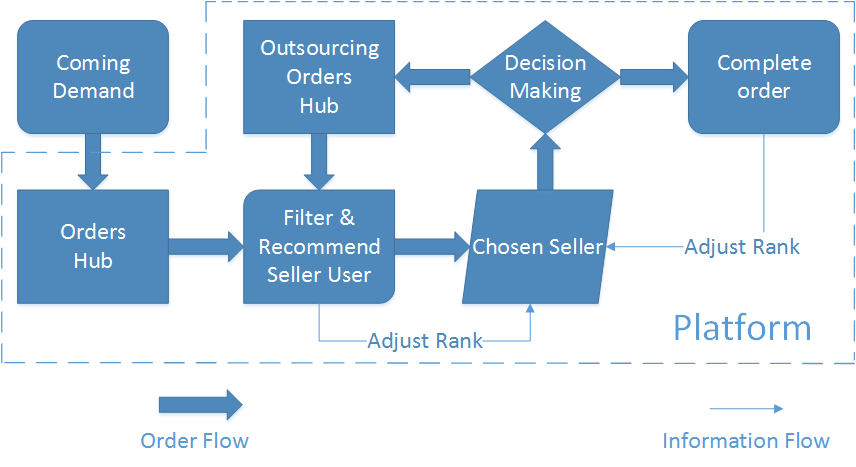
\includegraphics[width =\textwidth]{figures/wanting.png}
		\caption{The Ideal Model of the System}
	\end{figure}
}
\end{frame}

\subsection{Rating Schema}
\begin{frame}{Rating Schema}{Manufacturing Ecosystem Envolving}
\onslide<+->{Rating user's rank is the base of Recommand System, so the rating schema should be designed. Most modern rating systems are derived from Elo's model}
\onslide<+->{\begin{numcases}{}
E_A = \frac{1}{1+10^{\frac{R_B-R_A}{400}}} \\
R_A := R_A + K(S_A - E_A) \\
E_B = \frac{1}{1+10^{\frac{R_A-R_B}{400}}} \\
R_B := R_B + K(S_B - E_B)
\end{numcases}}
\end{frame}

\subsection{Recommand System}
\begin{frame}{Recommandation System}{Manufacturing Ecosystem Evolution}
\onslide<+->{There are two scenarios in recommendation:
\begin{itemize}
\item Service Searching
\item Platform priority setting
\end{itemize}
}
\onslide<+->{
	Collaboration Filtering is a popular method used in recommand system:
	\begin{equation}
	\begin{split}
	\min_{p_*,q_*,b_*} & \sum_{(u,i)\in\kappa}\left(r_{ui} -\mu - b_u - b_i - p^T_uq_i \right)^2 \\
		& + \lambda_3 \left( \|p_u\|^2 + \|q_i\|^2 + b_u^2 + b_i^2 \right)
	\end{split}
	\end{equation}
	\begin{numcases}{}
	\hat{r}_{ui} = b_{ui} + p^T_uq_i \\
	b_{ui} = \mu + b_u + b_i  \\
	\kappa =\{(u,i)|r_{ui} \text{is known}\}
	\end{numcases}
}
\end{frame}

\subsection{User Introduction \& Elimination}
\begin{frame}{User Introduction \& Elimination}{Manufacturing Ecosystem Envolving}
\onslide<+->{
	Ecosystem envolving need a good user introduction and elimination method with:
}
\onslide<+->{
	\begin{block}{Evolution}
	\begin{itemize}
	\item Reinforcement Learning
	\item Control
	\end{itemize}
	\end{block}
}
\end{frame}

\subsection{Envision of the Ecosystem}
\begin{frame}{Envision}{After a long running time and the system seems stable}
\onslide<+->{
	With poper scheduling and evolution, Cloud Manufacturing Ecosystem running with a stable mode:
	\begin{block}{Stable System Envision}
	\begin{itemize}
		\item Less-Popular manufacturing services are utilization instead of idleness with Coupon
		\item Products are manufactured with appropriate resources
		\item High rank users in different types of manufacturing resource lead the industrial chain
		\item Good operating models improved with time goes by
	\end{itemize}
	\end{block}
}
\end{frame}


\subsection{Simple Demo} % (fold)
\label{sub:simple_demo}
\begin{frame}{Simple Demo}
\only<1>{
Based on Elo model, we focus on the how sellers' ranks will
change with different specifications.

If we set $Q_A=10^{\frac{R_A}{400}}$ and $Q_B=10^{\frac{R_B}{400}}$, we have:
$$
\begin{cases}
E_A = \frac{Q_A}{Q_A + Q_B}\\
E_B = \frac{Q_B}{Q_B + Q_A}
\end{cases}
$$}
\only<2>{
For entity in the ecosystem(seller) $i,k$ ($i,k=1,2,\dots,n$), we assume that:
$$
\begin{cases}
Q_A = Q_i\\
Q_B = \frac{\sum_{k}\alpha_{ik}Q_k}{\sum_{k}\alpha_{ik}}
\end{cases}
$$
Where $\alpha_{ik}$ is the threating coefficient, the bigger the values is, the heigher $k$ threatens $i$.

\begin{center}
\href{localhost:8888}{\large Demo}
\end{center}
}
\end{frame}
% subsection simple_demo (end)
\iffalse
\subsection{Reinforcement Learning and Control} % (fold)
\label{sub:reinforcement_learning_and_control}
\begin{frame}{Aim}{Reinforcement Learning}
\begin{block}{The aim}
\begin{itemize}
	\item Uncover the right action for user
	\item Uncover the right action for administrator to make adjustments
	\item From the view of user
	\item From the view of industrial chain
\end{itemize}
\end{block}
\end{frame}

\begin{frame}{Main Parts}{Reinforcement Learning}
\begin{block}{Main parts and steps}
\begin{itemize}
	\item Define states
	\item Design actions
	\item Set reward function
	\item Design state simulation
	\item Simulate
\end{itemize}
\end{block}
\end{frame}
\fi

\section*{}
\begin{frame}
\centering
\Large
Thank You
\end{frame}
%% !TEX root = ../beamer.tex
\section*{Summary}

\begin{frame}{Summary}
  \begin{itemize}
  \item
    The \alert{first main message} of your talk in one or two lines.
  \item
    The \alert{second main message} of your talk in one or two lines.
  \item
    Perhaps a \alert{third message}, but not more than that.
  \end{itemize}
  
  \begin{itemize}
  \item
    Outlook
    \begin{itemize}
    \item
      Something you haven't solved.
    \item
      Something else you haven't solved.
    \end{itemize}
  \end{itemize}
\end{frame}





% All of the following is optional and typically not needed.
\iffalse
  \appendix
  \section<presentation>*{\appendixname}
  \subsection<presentation>*{bibliography}
  \begin{frame}[allowframebreaks]
    \tiny
    \frametitle<presentation>{bibliography}
    \nocite{*}
    \bibliography{references}
  \end{frame}
\fi
\end{document}
